% !TeX program = lualatex
\documentclass[fleqn]{NotesClass}

\strictpagecheck

\usepackage{csquotes}
\usepackage{subcaption}

\usepackage{tikz}
\usetikzlibrary{external}
\tikzexternalize[prefix=tikz-external/]

\usepackage{tikz-cd}
\AtBeginEnvironment{tikzcd}{\tikzexternaldisable}
\AtEndEnvironment{tikzcd}{\tikzexternalenable}

\usepackage[pdfauthor={Willoughby Seago},pdftitle={Notes from Algebraic Geometry Course},pdfkeywords={algebraic geometry},pdfsubject={Algebraic Geometry}]{hyperref}  % Should be loaded second last (cleveref last)
\colorlet{hyperrefcolor}{blue!60!black}
\hypersetup{colorlinks=true, linkcolor=hyperrefcolor, urlcolor=hyperrefcolor}
\usepackage[
capitalize,
nameinlink,
noabbrev
]{cleveref} % Should be loaded last

% My packages
\usepackage{NotesBoxes}
\usepackage{NotesMaths2}

\setmathfont[range={\int, \oint, \otimes, \oplus, \bigotimes, \bigoplus}]{Latin Modern Math}


% Highlight colour
\definecolor{my blue}{HTML}{084887}
\definecolor{my red}{HTML}{CA1551}
\definecolor{my green}{HTML}{17C3B2}
\definecolor{my yellow}{HTML}{F58A07}
\definecolor{my purple}{HTML}{CB9CF2}
\colorlet{highlight}{my green}

% Title page info
\title{Algebraic Geometry}
\author{Willoughby Seago}
\date{October 6th, 2025}
\subtitle{Notes from}
\subsubtitle{University of Glasgow}
\renewcommand{\abstracttext}{These are my notes from the SMSTC course \emph{Algebraic Geometry} taught by Dr Giulia Gugiatti and Prof Ivan Cheltsov. The lectures, and hence these notes, follow the \textit{Algebraic Geometry} notes of Andreas Gathmann. These notes were last updated at \printtime{} on \today{}.}

% Commands
% Maths
\newcommand{\subideal}{\trianglelefteq}
\newcommand{\affine}{\symbb{A}}

\includeonly{appendices/comm-alg}

\begin{document}
    \frontmatter
    \titlepage
    \innertitlepage{}
    \tableofcontents
    % \listoffigures
    \mainmatter
    
    \chapter{Introduction}
    
    \section{Conventions and Notation}
    Throughout the notes the ground field, \(K\), will always be assumed to be \emph{algebraically closed}, up to the point where we introduce schemes.
    Taking \(K = \complex\) is usually reasonable.
    
    All rings, \(R\), are assumed to be \emph{commutative} with \emph{unity}.
    That \(J\) is an ideal of \(R\) will be denoted \(J \subideal R\).
    The ideal generated by a subset, \(S \subseteq R\), is denoted \(\langle S \rangle\).
    
    We write \(K[x_1, \dotsc, x_n]\) for the ring of polynomials with coefficients in \(K\) in the variables \(x_1, \dotsc, x_n\).
    We write \(f(a)\) to mean the evaluation of an element of this ring at the point \(a = (a_1, \dotsc, a_n) \in K^n\), and where no confusion may arise we'll usually call this point \(x = (x_1, \dotsc, x_n)\).
    
    \section{Motivation}
    This section contains various motivating examples of algebro-geometric thinking, in varying levels of precision.
    Since the goal is to motivate some precision may be lacking.
    
    \subsection{Systems of Polynomial Equations}
    When we first learned algebra in high school it was to study the zeros of polynomials.
    Later we learned linear algebra, which it can be argued is the study of the zeros of systems of linear equations.
    Algebraic geometry combines these two fundamental fields into the study of zeros of systems of polynomials.
    
    Given \(f_1, \dotsc, f_m \in K[x_1, \dotsc, x_n]\) the basic object of study of algebraic geometry is the \defineindex{affine variety}
    \begin{equation}
        X = \{x \in K^n \mid f_i(x) = 0 \text{ for } i = 1, \dotsc, m\}.
    \end{equation}
    What questions can we ask about this set?
    Just as a single complex polynomial, \(f \in \complex[x]\), cannot be solved exactly for \(\deg f > 4\) we cannot possibly hope to explicitly list the points in \(X\).
    Instead we reason about the geometric structure of the solutions.
    We will ask geometric questions about \(X\), which we then aim to answer by an algebraic study of the \(f_i\).
    
    In the following sections we will give several examples of the sorts of geometric objects which can arise.
    We will focus on the existence of connections to other areas of mathematics.
    
    \subsection{Riemann Surfaces}
    Fix some positive integer, \(n\).
    We can define a curve\footnote{Note that this is a \enquote{curve} since it's complex dimension is \(1\) (we'll define dimension of affine varieties later, for now just use your intuition for the dimension of a manifold). Of course, in our pictures this single complex dimension is drawn as two real dimensions.}
    \begin{equation}
        c_n = \{(x, y) \in \complex^2 \mid y^2 = (x - 1)(x - 2)(x - 3) \dotsm (x - 2n)\} \subseteq \complex^2.
    \end{equation}
    We can view the defining equation as defining the quantity \(y\).
    Since we have \(y^2 = \dotso\) to find the value of \(y\) we have to take a square root.
    What we get depends on the value of \(x\).
    For most cases, specifically \(x \ne 1, 2, \dotsc, 2n\), we have
    \begin{equation}
        y = \pm \sqrt{(x - 1)(x - 2) \dotsm (x - 2n)}.
    \end{equation}
    For \(x = 1, 2, \dotsc, 2n\) we have
    \begin{equation}
        y = 0.
    \end{equation}
    Consider what values \(y\) can take.
    For \(x \ne 1, \dotsc, 2n\) we have two copies of \(\complex\), one for \(+ \sqrt{(x-1) \dotsm (x - 2n)}\) and one for \(-\sqrt{(x - 1) \dotsm (x - 2n)}\).
    For \(x = 1, \dotsc, 2n\) we only have one possible value, \(0\).
    The picture this suggests is two copies of \(\complex\) identified at the points \(1, \dotsc, 2n\).
    
    However, this isn't quite right.
    We know that \(z \in \complex^{\times}\) doesn't have a distinguished choice of \(\sqrt{z}\).
    Upon passing once around the origin they are exchanged.
    For example, if we take the path \(x = r\e^{i\theta}\), with \(r \ge 0\) fixed and \(\theta \in [0, 2\pi]\) then \(\sqrt{x} = \sqrt{r} \e^{i\theta/2}\).
    Then at \(\theta = 0\) we get \(\sqrt{r}\) and at \(\theta = 2\pi\) we get \(-\sqrt{r}\).
    The result is that as we go around the points \(x = 1, \dotsc, 2n\) we move from one copy of \(\complex\) to the other.
    
    Fortunately, we know how to deal with this, we take branch cuts between zeros.
    Take both copies of \(\complex\), and perform branch cuts along the intervals \([1, 2], [3, 4], \dotsc, [2n - 1, 2n]\).
    For \(n = 3\) this produces \cref{fig:complex planes with branch cuts}.
    Now glue these along the cuts, which gives the picture
    % TODO
    Finally, because it makes things nicer, add two points at infinity, one for each copy of \(\complex\), compactifying everything to get the picture
    % TODO
    We see that this leaves us with a Riemann surface of genus \(g = n - 1\).
    This relates algebraic geometry to the theory of Riemann surfaces.
    
    \begin{figure}
        \centering
        \begin{subfigure}{0.8\textwidth}
            \tikzexternaldisable
            \tikzsetnextfilename{riemann-surface-1}
            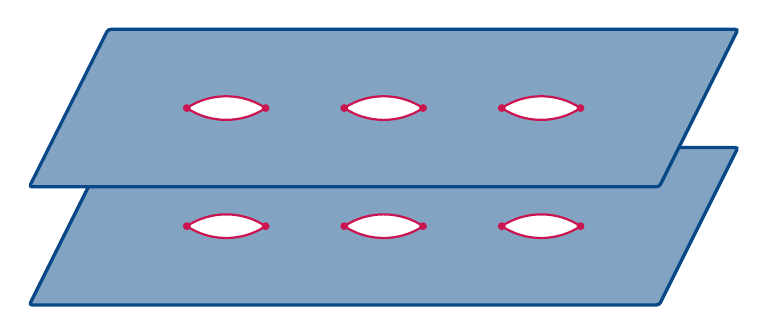
\begin{tikzpicture}
                \draw [very thick, rounded corners=1, my blue, fill=my blue!50] (0, -2) -- (8, -2) -- (9, 0) -- (1, 0) -- cycle;
                \draw [very thick, rounded corners=1, my blue, fill=my blue!50] (0, -0.5) -- (8, -0.5) -- (9, 1.5) -- (1, 1.5) -- cycle;
                
                \foreach \i in {1, 3, 5} {
                    \fill [white]  (1 + \i, 0.5) .. controls (1.3 + \i, 0.7) and (1.7 + \i, 0.7) .. (2 + \i, 0.5) .. controls (1.7 + \i, 0.3) and (1.3 + \i, 0.3) .. (1 + \i, 0.5);
                    \fill [white] (1 + \i, -1) .. controls (1.3 + \i, -0.8) and (1.7 + \i, -0.8) .. (2 + \i, -1) .. controls (1.7 + \i, -1.2) and (1.3 + \i, -1.2) .. (1 + \i, -1);
                    \draw [thick, my red] (1 + \i, 0.5) .. controls (1.3 + \i, 0.7) and (1.7 + \i, 0.7) .. (2 + \i, 0.5);
                    \draw [thick, my red] (1 + \i, 0.5) .. controls (1.3 + \i, 0.3) and (1.7 + \i, 0.3) .. (2 + \i, 0.5);
                    \draw [thick, my red] (1 + \i, -1) .. controls (1.3 + \i, -0.8) and (1.7 + \i, -0.8) .. (2 + \i, -1);
                    \draw [thick, my red] (1 + \i, -1) .. controls (1.3 + \i, -1.2) and (1.7 + \i, -1.2) .. (2 + \i, -1);
                }
                \foreach \i in {1, 2, 3, 4, 5, 6} {
                    \fill [my red] (1 + \i, 0.5) circle [radius=0.05];
                    \fill [my red] (1 + \i, -1) circle [radius=0.05];
                }
            \end{tikzpicture}
            \caption{Branch cuts along alternate intervals.}
            \label{fig:complex planes with branch cuts}
        \end{subfigure}
        \caption{Producing a Riemann surface from a curve}
    \end{figure}
    
    We can change our curve to
    \begin{equation}
        \{(x, y) \in \complex^2 \mid y^2 = (x - 1)^2(x - 2)(x - 3) \dotsm (x - 2n)\} \subseteq \complex^2.
    \end{equation}
    Then the same analysis can be applied, except that we have a singular point at the repeated root, \(x = 1\).
    This relates algebraic geometry to singularity theory.
    
    \subsection{Lines on Spaces}
    Consider the surface
    \begin{equation}
        X = \{(x_1, x_2, x_3) \in \reals^3 \mid 1 + x_1^3 + x_2^3 + x_3^3 - (1 + x_1 + x_2 + x_3)\} \subseteq \reals^3.
    \end{equation}
    This is called the \defineindex{Clebsch surface}.
    This is a cubic surface because it's defined by a single cubic equation.
    It's possible to draw straight lines on this surface.
    One can ask how many such straight lines exist.
    The answer, surprisingly, is always 27, at least under some mild conditions.
    Cubic surfaces are actually a weird middle ground, between the infinite families of lines on a quadratic surface, and the general absence of lines on surfaces defined by any higher degree equation.
    
    The question of how many geometric objects of a certain type exist is one of enumerative geometry, which makes heavy use of algebraic geometry.
    
    \subsection{String Theory}
    Strings, world sheets, those are surfaces, physicists should care about algebraic geometry.
    
    \subsection{Curves in Space}
    Consider the following curve
    \begin{equation}
        X = \{(x_1, x_2, x_3) = (t^3, t^4, t^5) \mid t \in \complex\} \subseteq \complex^3.
    \end{equation}
    This is a parametric definition of this surface.
    We can equally define it explicitly as
    \begin{equation}
        X = \{(x_1, x_2, x_3) \mid x_1^3 = x_2x_3, x_2^2 = x_1x_3, x_3^2 = x_1^2x_2\} \subseteq \complex^3.
    \end{equation}
    This is a surface, so it's two (complex) dimensional.
    However, we need all three of these equations to define it, if we remove any of them we don't get the same surface.
    This is very different to the world of linear algebra, where we'd have linear defining relations.
    There any codimension \(d\) subspace can be defined by \(d\) (linear) equations.
    Here \(X\) is one-dimensional, so it has codimension \(2\), but we need three equations to define it.
    
    The general problem of taking an affine variety, \(X\), defined as the vanishing set of some polynomials, and determining its dimension is actually very hard.
    We can use Gr\"obner bases to do this, but the algebra is pretty unwieldy, and we're forced to use computers to solve it most of the time.
    A Gr\"obner basis is a certain generating set of the ideal generated by the polynomials defining the affine variety.
    Actually, even defining dimension for an arbitrary affine variety is not that straight forward, but for now the intuition from manifolds and vector spaces should be enough.
    
    \subsection{Different Fields}
    Over \(\reals\) or \(\complex\) we can use real or complex analytic methods to study the zeros of polynomials, and hence affine varieties.
    
    Over \(\rationals\) or finite fields we can use number theoretic techniques to study the zeros of polynomials, and hence affine varieties.
    
    For example, Fermat's last theorem can be stated as the study of the affine variety
    \begin{equation}
        X = \{(x_1, x_2, x_3) \in \rationals^3 \mid x_1^n + x_2^n = x_3^n\},
    \end{equation}
    where the question we ask is if this has any non-trivial points.
    
    \chapter{Affine Varieties}
    \section{Affine Varieties}
    \begin{dfn}{Affine Space}{}
        \define{Affine \(\symbb{n}\)-space}\index{affine n-space@affine \(n\)-space} over \(K\) is the set
        \begin{equation}
            \affine^n = \affine_K^n \coloneq \{(a_1, \dotsc, a_n) \mid a_i \in K \forall i = 1, \dotsc, n\}.
        \end{equation}
    \end{dfn}
    
    Note that as sets \(\affine^n = K^n\).
    However, we write \(\affine^n\) when we wish to forget the additional algebraic structure of \(K^n\), specifically the vector space and ring, that is, we want to forget about the ability to scale, add and multiply elements.
    
    For the time being we will take \(\affine^n\) as our ambient space.
    Then a polynomial, \(f \in K[x_1, \dotsc, x_n]\), defines a \defineindex{polynomial function}
    \begin{align}
        \affine^n &\to K\\
        a &\mapsto f(a).
    \end{align}
    We'll usually call this function \(f\) as well.
    
    \begin{dfn}{Affine Variety}{}
        Let \(S \subseteq K[x_1, \dotsc, x_n]\) be some set of polynomials.
        The \defineindex{zero locus} or \defineindex{vanishing set} of \(S\), denoted \(V(S)\), is all points of \(\affine^n\) on which the polynomial functions defined by polynomials in \(S\) vanish.
        That is,
        \begin{equation}
            V(S) \coloneq \{x \in \affine^n \mid f(x) = 0 \forall f \in S\} \subseteq \affine^n
        \end{equation}
        Any subset of \(\affine^n\) of this form is called an \defineindex{affine variety}.
    \end{dfn}
    
    \begin{wrn}
        Note that some authors require that affine varieties have the additional property of being irreducible.
        These authors would then call all sets like \(V(S)\) \define{affine algebraic sets}\index{affine algebraic set}.
    \end{wrn}
    
    \begin{ntn}{}{}
        If \(S = \{f_1, \dotsc, f_n\}\) is a finite set we write
        \begin{equation}
            V(S) = V(\{f_1, \dotsc, f_n\}) = V(f_1, \dotsc, f_n).
        \end{equation}
    \end{ntn}
    
    There are some properties we can immediately prove about affine varieties.
    
    \begin{lma}{Reversal of Inclusion}{lma:V reverses inclusion}
        If \(S_1 \subseteq S_2 \subseteq K[x_1, \dotsc, x_n]\) then \(V(S_2) \subseteq V(S_1)\).
        \begin{proof}
            Suppose \(x \in V(S_2)\).
            Then \(f(x) = 0\) for all \(f \in S_2\), and so certainly \(f(x) = 0\) for \(f \in S_1 \subseteq S_2\), and thus \(x \in V(S_1)\).
        \end{proof}
    \end{lma}
    
    \begin{lma}{Union}{lma:union of defining equations}
        If \(S_1, S_2 \subseteq K[x_1, \dotsc, x_n]\) then \(V(S_1) \cup V(S_2) = V(S_1 S_2)\) where
        \begin{equation}
            S_1 S_2 = \{fg \mid f \in S_1, g \in S_2\}.
        \end{equation}
        \begin{proof}
            We start by showing that \(V(S_1) \cup V(S_2) \subseteq V(S_1 S_2)\).
            Suppose that \(x \in V(S_1) \cup V(S_2)\).
            Then \(x \in V(S_1)\), so \(f(x) = 0\) for all \(f \in S_1\), and \(x \in V(S_2)\), so \(g(x) = 0\) for all \(g \in S_2\).
            Thus, for \(f \in S_1\) and \(g \in S_2\) we have \((fg)(x) = f(x)g(x) = 0 \cdot 0 = 0\), so \(x \in V(S_1S_2)\).
            
            We now show that \(V(S_1S_2) \subseteq V(S_1) \cup V(S_2)\).
            We do so by supposing that \(x \notin V(S_1) \cup V(S_2)\).
            Then there exist polynomials, \(f \in S_1\) and \(g \in S_2\), for which \(f(x) \ne 0\) and \(g(x) \ne 0\).
            Thus, \((fg)(x) = f(x)g(x) \ne 0\) (since we work in a field, so have no nonzero zero divisors).
            Thus, \(x \notin V(S_1S_2)\) since \(fg \in S_1S_2\).
            By the contrapositive then we have that if \(x \in V(S_1S_2)\) then \(x \in V(S_1) \cup V(S_2)\).
        \end{proof}
    \end{lma}
    
    \begin{lma}{Intersection}{lma:intersection of defining equatinos}
        Let \(J\) be an index set, and \(\{S_j\}_{j \in J}\) an indexed family of subsets of \(K[x_1, \dotsc, x_n]\).
        Then
        \begin{equation}
            \bigcap_{j \in J} V(S_j) = V\left( \bigcup_{j \in J} S_j \right).
        \end{equation}
        \begin{proof}
            Suppose \(x \in \bigcap_{j \in J} V(S_j)\).
            Then \(x \in V(S_j)\) for all \(j \in J\).
            Thus, \(f(x) = 0\) for all \(f \in S_j\) for all \(j \in J\).
            Thus, \(x \in V\left( \bigcup_{j \in J} S_j \right)\).
            
            Conversely, suppose \(x \in V\left( \bigcup_{j \in J} S_j \right)\).
            Then \(f(x) = 0\) for all \(f \in \bigcup_{j \in J} S_j\), which means \(f(x) = 0\) for all \(f \in S_j\) for any \(j \in J\), and therefore \(x \in \bigcap_{j \in J} V(S_j)\).
        \end{proof}
    \end{lma}
    
    We can also give some examples of simple affine varieties.
    
    \begin{exm}{Affine Varieties}{}
        \begin{enumerate}
            \item Affine \(n\)-space is itself an affine variety.
            Specifically, \(\affine^n = V(0)\), since the zero polynomial vanishes.
            \item The empty set is an affine variety.
            Specifically, \(\emptyset = V(1)\), since the constant polynomial at \(1\) vanishes nowhere.
            \item Any linear subspace of \(K^n = \affine^n\) is an affine variety since a linear subspace is defined by the vanishing of linear equations.
            \item If \(X \subseteq \affine^n\) and \(Y \subseteq \affine^m\) are affine varieties then \(X \times Y\) is too when viewed as a subspace of \(\affine^{m + n}\).
            The defining equations of \(X \times Y\) are those of \(X\) and \(Y\) where we view those of \(X\) as a function of \(x_1, \dotsc, x_m\) and those of \(Y\) as a function of \(x_{m + 1}, \dotsc, x_{m + n}\).
        \end{enumerate}
    \end{exm}
    
    \begin{remark}{}{}
        The above results say that \(\emptyset\) and \(\affine^n\) are both affine varieties, and that affine varieties are closed under finite union and arbitrary intersections.
        This is very close to the definition of a topology on \(\affine^n\) in terms of open sets, \(\emptyset\) and \(X\) should be open, and the topology should be closed under finite intersections and arbitrary unions.
        Notice how unions and intersections exchange roles.
        Instead what we have is actually the requirements to define a topology on \(\affine^n\) via the \emph{closed} sets.
        We'll do exactly this in . % TODO add reference to section on Zarisiki topology
    \end{remark}
    
    \begin{exm}{Affine \(1\)-Space}{}
        The only affine varieties in \(\affine^1\) are \(\affine^1\), \(\emptyset\), and all finite sets.
        Any finite set, \(\{\alpha_1, \dotsc, \alpha_n\}\), is the vanishing set of \((x - \alpha_1) \dotsm (x - \alpha_n)\).
        To show that infinite sets cannot be affine varieties here (other than \(\affine^1\)) suppose \(X = V(S)\) is infinite for some \(S \subseteq K[x]\).
        Fix some \(f \in S\).
        Then \(\{f\} \subseteq S\), so by \cref{lma:V reverses inclusion} \(V(S) \subseteq V(f)\), and so \(x \in V(f)\) for all \(x \in X\), which means that \(f(x) = 0\) for all \(x \in X\), and so \(f\) has infinitely many roots, which is not possible for a polynomial.
    \end{exm}
    
    If \(f, g \in K[x_1, \dotsc, x_n]\) vanish on \(X \subseteq \affine^n\) then so do \(f + g\) and \(f h\) for any \(h \in K[x_1, \dotsc, x_n]\).
    Thus, the set, \(S\), defining an affine variety, \(X = V(S)\), is certainly not unique.
    We can always add \(f + g\) and \(fh\).
    From this we see that \(V(S) = V(\langle S \rangle)\) where \(\langle S \rangle \subideal K[x_1, \dotsc, x_n]\) is the ideal generated by \(S\).
    This means that any affine variety can be expressed as the vanishing set of some ideal of a polynomial ring.
    
    Hilbert's basis theorem (\cref{thm:hilberts basis theorem,crl:poly ring over noetherian is noetherian}) along with a standard characterisation of noetherian rings (\cref{lma:noetherian iff all ideals finitely generated}) tells us that all ideals of \(K[x_1, \dotsc, x_n]\) are finitely generated.
    Given an affine variety, \(X = V(S)\), we can then take \(X = V(\langle S \rangle)\), and then we can find some finite generating set for this ideal, \(S'\).
    Then \(X = V(S')\).
    Thus, every affine variety is the zero locus of a finite set of polynomials.
    
    \begin{dfn}{Radical}{}
        Let \(R\) be a ring with ideal \(J\).
        The \defineindex{radical} of \(J\) is
        \begin{equation}
            \sqrt{J} = \{f \in R \mid f^k \in J \text{ for some } k \in \naturals\}.
        \end{equation}
        We say \(J\) is \define{radical} if \(J = \sqrt{J}\).
    \end{dfn}
    
    \begin{lma}{}{lma:ideal is subset of its radical}
        Let \(J \subideal R\).
        Then \(J \subseteq \sqrt{J}\).
        \begin{proof}
            Suppose that \(f \in J\), then \(f^1 \in J\), and so \(f \in \sqrt{J}\).
        \end{proof}
    \end{lma}
    
    We can now state some results which are the analogues of \cref{lma:V reverses inclusion,lma:union of defining equations,lma:intersection of defining equatinos} when we work with zero loci of ideals.
    
    \begin{lma}{}{}
        Let \(J \subideal K[x_1, \dotsc, x_n]\).
        Then \(V(\sqrt{J}) = V(J)\).
        \begin{proof}
            First, \cref{lma:ideal is subset of its radical} gives us \(J \subseteq \sqrt{J}\).
            Thus, by \cref{lma:V reverses inclusion} we have that \(V(\sqrt{J}) \subseteq V(J)\).
            
            Now suppose that \(x \in V(J)\) and \(f \in \sqrt{J}\).
            Then \(f^k \in J\), so \(f^k(x) = 0\), and since we're in a field with no nonzero zero divisors we must have that \(f(x) = 0\), and so \(x \in V(\sqrt{J})\).
        \end{proof}
    \end{lma}
    
    This result, combined with our earlier analysis, means that every affine variety is the zero locus of a radical ideal.
    
    \begin{lma}{Union}{}
        If \(J_1, J_2 \subideal K[x_1, \dotsc, x_n]\) then \(V(J_1) \cup V(J_2) = V(J_1 J_2) = V(J_1 \cap J_2)\).
        \begin{proof}
            That \(V(J_1) \cup V(J_2) = V(J_1 J_2)\) is \cref{lma:union of defining equations}.
            It remains to show that \(V(J_1 J_2) = V(J_1 \cap J_2)\).
            Note that it is not generally true that \(J_1 J_2 \stackrel{!}{=} J_1 \cap J_2\).
            However, it is true that \(\sqrt{J_1J_2} = \sqrt{J_1 \cap J_2}\) (\cref{lma:radical of product is radical of intersection}), and the result follows from this.
        \end{proof}
    \end{lma}
    
    \begin{lma}{Intersection}{}
        If \(J_1, J_2 \subideal K[x_1, \dotsc, x_n]\) then \(V(J_1) \cap V(J_2) = V(J_1 + J_2)\).
        \begin{proof}
            From \cref{lma:intersection of defining equatinos} we have that \(V(J_1) \cap V(J_2) = V(J_1 \cup J_2)\).
            We also have that \(\langle J_1 \cup J_2 \rangle = J_1 + J_2\), so \(V(J_1 \cup J_2) = V(\langle J_1 \cup J_2 \rangle) = V(J_1 + J_2)\).
        \end{proof}
    \end{lma}
    
    \begin{remark}{}{}
        With these results we have set up a pairing between geometric objects and algebraic objects.
        Specifically, we've defined a map
        \begin{align}
            V \colon \{\text{algebraic objects}\} &\to \{\text{geometric objects}\}\\
            \text{ideal} &\mapsto \text{affine variety}.
        \end{align}
        Studying the map going in the opposite direction will be the focus of the next section.
    \end{remark}
    
    \section{Ideal of an Affine Variety}
    \begin{dfn}{Ideal}{}
        Let \(X\) be a subset of \(\affine^n\).
        The \defineindex{ideal} of \(X\) is
        \begin{equation}
            I(X) \coloneq \{f \in K[x_1, \dotsc, x_n] \mid f(x) = 0 \forall x \in X\}.
        \end{equation}
    \end{dfn}
    
    This is indeed an ideal, if \(f, g \in I(X)\) then \(f(x) = g(x) = 0\) for all \(x \in X\) and \(f(x) + g(x) = 0\), so \(f + g \in I(X)\), and \(-f(x) = 0\) so \(-f \in I(X)\), and if \(h \in K[x_1,\dotsc, x_n]\) then \(f(x)h(x) = 0h(x) = 0\) so \(fh \in I(X)\).
    
    \begin{lma}{Reversal of Inclusion}{}
        Suppose \(X_1 \subseteq X_2 \subseteq \affine^n\).
        Then \(I(X_2) \subseteq I(X_1)\).
        \begin{proof}
            Suppose that \(f \in I(X_2)\), that is, \(f(x) = 0\) for all \(x \in X_2\).
            Then \(f(x) = 0\) for all \(x \in X_1 \subseteq X_2\), and so \(f \in I(X_1)\).
        \end{proof}
    \end{lma}
    
    \begin{lma}{Ideal is Radical}{}
        If \(X \subseteq \affine^n\) then \(I(X)\) is radical.
        \begin{proof}
            Suppose \(f \in \sqrt{I(X)}\).
            Then \(f^k \in I(X)\) for some \(k \in \naturals\).
            Then \(f^k(x) = 0\) for all \(x \in X\), and since we're in a field \(f(x) = 0\) for all \(x \in X\), and thus \(f \in I(X)\), and hence \(\sqrt{I(X)} \subseteq I(X)\).
            We also have \(I(X) \subseteq \sqrt{I(X)}\) by \cref{lma:ideal is subset of its radical}.
            Thus, \(I(X) = \sqrt{I(X)}\).
        \end{proof}
    \end{lma}
    
    \begin{remark}{}{}
        This gives us the other side of the pairing between algebraic objects and geometric objects:
        \begin{equation}
            I \colon \{\text{subsets of } \affine^n\} \to \{\text{radical ideals of } K[x_1, \dotsc, x_n]\}.
        \end{equation}
        These aren't quite inverses, since in this direction we only produce radical ideals.
        However, as we've seen radical ideals are good enough if we're applying \(V\).
        The following important theorem tells us that these maps, while not quite inverses, are essentially inverses, so long as we're happy to only deal with radical ideals, which we can do by liberally taking radicals.
    \end{remark}
    
    \begin{thm}{Hilbert's Nullstellensatz}{}
        \begin{enumerate}
            \item For any affine variety, \(X \subseteq \affine^n\), we have \(V(II(X)) = X\).
            \item For any ideal, \(J \subideal K[x_1, \dotsc, x_n]\), we have \(I(V(J)) = \sqrt{J}\).
        \end{enumerate}
        \begin{proof}
            We first prove that \(X \subseteq V(I(X))\).
            If \(x \in X\) then \(f(x) = 0\) for all \(f \in I(X)\), and thus \(x \in V(I(X))\).
            
            Next, we prove that \(\sqrt{J} \subseteq I(V(J))\).
            If \(f \in \sqrt{J}\) then \(f^k \in J\) for some \(k \in \naturals\).
            Thus, \(f^k(x) = 0\) for all \(x \in V(J)\), and so \(f(x) = 0\) for all \(x \in V(J)\), and so \(f \in I(V(J))\).
            
            Third, we prove that \(V(I(X)) \subseteq X\).
            Since \(X\) is an affine variety we know that there is some ideal, \(J \subideal K[x_1, \dotsc, x_n]\), for which \(X = V(J)\).
            Then \(\sqrt{J} \subseteq I(V(J))\) by the previous step, and \(J \subseteq \sqrt{J}\), so \(J \subseteq I(V(J))\).
            Taking the zero locus, which reverses the inclusion (\cref{lma:V reverses inclusion}), we have \(V(I(V(J))) \subseteq V(J)\).
            Since \(X = V(J)\) this is then exactly \(V(I(X)) \subseteq X\), and so combined with the first step we have that \(V(I(X)) = X\).
            
            The only hard step of the proof is showing that \(I(V(J)) \subseteq \sqrt{J}\).
            This requires some pretty heavy commutative algebra, so we'll skip it.
        \end{proof}
    \end{thm}
    
    \begin{remark}{}{}
        Nullstellensatz means \enquote{theorem of the zeroes}.
    \end{remark}
    
    
    \appendixpage
    \begin{appendices}
        \chapter{Commutative Algebra}
Here we collect some results from commutative algebra which we'll make use of in the course.
This won't be very well organised, and is more for reference than actual reading.
The conditions to be included here are pretty much \enquote{I had to look it up} or \enquote{I had to think about it for more than 10 seconds} while writing these notes, or \enquote{I thought it was worth recapping}.

\section{Ideals}

\begin{dfn}{Prime Ideal}{}
    A proper ideal, \(\ideal{p} \subideal R\), is \define{prime}\index{prime ideal} if whenever \(ab \in \ideal{p}\) for \(a, b \in R\) then either \(a \in \ideal{p}\) or \(b \in \ideal{p}\).
    
    Equivalently, \(\ideal{p}\) is prime if \(R/\ideal{p}\) is an integral domain.
\end{dfn}

\begin{dfn}{Maximal Ideal}{}
    A proper ideal, \(\ideal{m} \subideal R\), is \define{maximal}\index{maximal ideal} if whenever there is another ideal, \(I \subideal R\), with \(\ideal{m} \subseteq I\) then either \(I = \ideal{m}\) or \(I = R\).
    
    Equivalently, \(\ideal{m}\) is maximal if \(R/\ideal{m}\) is a field.
\end{dfn}

\begin{lma}{}{lma:product of ideals subset of intersection}
    Let \(R\) be a ring with ideals \(I\) and \(J\).
    Then \(IJ \subseteq I \cap J\).
    \begin{proof}
        If \(a \in I\) and \(b \in J\) then \(ab \in I\) and \(ab \in J\) by definition of an ideal.
        Then \(ab \in I \cap J\).
    \end{proof}
\end{lma}

\begin{lma}{}{lma:radical of product is radical of intersection}
    Let \(R\) be a ring with ideals \(I\) and \(J\).
    Then \(\sqrt{IJ} = \sqrt{I \cap J} = \sqrt{I} \cap \sqrt{J}\).
    \begin{proof}
        We prove a circle of inclusions.
        We start with \(\sqrt{IJ} \subseteq \sqrt{I \cap J}\), which follows from \cref{lma:product of ideals subset of intersection}.
        
        If \(a \in \sqrt{I \cap J}\) then \(a^k \in I \cap J\) for some \(k \in \naturals\).
        Thus, \(a^k \in I\) and \(a^k \in J\).
        Hence, \(a \in \sqrt{I} \cap \sqrt{J}\).
        
        If \(a \in \sqrt{I} \cap \sqrt{J}\) then \(a^k \in I\) and \(a^{\ell} \in J\) for some \(k, \ell \in \naturals\).
        Then \(a^k a^{\ell} = a^{k + \ell} \in IJ\), and so \(a \in \sqrt{IJ}\).
    \end{proof}
\end{lma}

\begin{lma}{}{lma:prime ideal is radical}
    Every prime ideal is radical.
    \begin{proof}
        Let \(\ideal{p}\) be a prime ideal of a ring, \(R\).
        Consider \(\sqrt{\ideal{p}}\).
        If \(a \in \sqrt{\ideal{p}}\) then there exists some \(k \in \naturals\) such that \(a^k \in \ideal{p}\).
        Suppose that \(k\) is minimal in making this true.
        If \(k = 1\) then \(a \in \ideal{p}\).
        If \(k > 1\) then by the definition of a prime ideal have \(x \cdot x^{k-1} \in \ideal{p}\) implying \(x \in \ideal{p}\) or \(x^{k-1} \in \ideal{p}\).
        However, the later cannot be the case because \(k\) was assumed minimal.
        Therefore, \(x \in \ideal{p}\), and since \(\ideal{p} \subseteq \sqrt{\ideal{p}}\) (\cref{lma:ideal is subset of its radical}) it must be that \(\ideal{p} = \sqrt{\ideal{p}}\).
    \end{proof}
\end{lma}

\section{Noetherian Rings}
\begin{dfn}{Noetherian}{}
    A ring, \(R\), is noetherian if it satisfies the ascending chain condition.
    That is, if every chain of ideals,
    \begin{equation}
        I_1 \subseteq I_2 \subseteq I_3 \subseteq \dotsb
    \end{equation}
    terminates, so \(I_{n+1} = I_n\) for sufficiently large \(n\).
\end{dfn}

Note that all fields are noetherian, and so is \(\integers\).

\begin{lma}{}{lma:noetherian iff all ideals finitely generated}
    Let \(R\) be a ring.
    The following are equivalent:
    \begin{enumerate}
        \item \(R\) is a noetherian.
        \item Every ideal of \(R\) is finitely generated.
    \end{enumerate}
\end{lma}

\subsection{Hilbert's Basis Theorem}
\begin{thm}{Hilbert's Basis Theorem}{thm:hilberts basis theorem}
    If \(R\) is a noetherian ring then \(R[x]\) is also Noetherian.
\end{thm}

\begin{crl}{}{crl:poly ring over noetherian is noetherian}
    If \(R\) is a noetherian ring then \(R[x_1, \dotsc, x_n]\) is noetherian.
\end{crl}


    \end{appendices}
    \backmatter
    \renewcommand{\glossaryname}{Acronyms}
    \printglossary[acronym]
    \printindex
\end{document}